\section{Diagnosing the Causes of Softmax Collapse}
\label{sec:nlm}

In the previous section we have shown that FP errors arise due to a combination of low losses and large logits, and shown that when FP errors are mitigated, grokking can be observed in conditions where it previously was not. In this section, we dive deeper and ask why extremely low losses and large logits appear in the first place in grokking tasks. We identify two main causes for this tendency: (i) easiness of overfitting in grokking tasks, and (ii) a training dynamic that sees gradients align with what we call \textit{naïve loss minimization} direction. After diagnosing the causes, the following section will use these insights to develop an optimization algorithm that avoids NLM in the first place.

\subsection{Ease of overfitting in grokking tasks}

The first important characteristic of grokking tasks that lead to SC is their ease of overfitting. It has been observed that as grokking datasets get larger, overfitting becomes harder, eventually leading to a regime where train and test performances increase in tandem \citep{power2022grokking, Nanda2023-hf, Varma2023}. It has also been shown that generalization can be delayed in the Sparse Parity task by increasing the amount of noise in the input, which makes overfitting easier \citep{Barak2022-el}. Here we investigate the opposite effect: that by decreasing the dimensionality of the input the data becomes harder to memorize, removing the delay in generalization.

To do this, we investigate the common grokking task of modular addition, but instead of the high-dimensional one-hot representations of the input integers, we use a more compact binary. More specifically, we assign each integer a distinct random binary vector of dimension 14.

Results confirm our hypothesis, showing that as input representations are decreased in dimension, overfitting is prevented and models generalize without need for regularization (\cref{fig:input_representations}, right). This also shows that modular addition only induces grokking depending on the choice of representation. These findings highlight the importance of understanding the training dynamics beyond the point of overfitting (i.e. point of achieving 100\% training accuracy), rather than focusing on the specifics of the modular arithmetic tasks as the key to explaining the delay in generalization.


\subsection{Naïve loss minimization}

We next identify a crucial training dynamic that commonly occurs in grokking tasks as a central cause for increasing logits and SC. We find that after reaching 100\% training accuracy, gradient updates are dominated by an update direction we term \textit{naïve loss minimization} (NLM). This direction does not change the model's decision boundary, but still decreases loss by simply scaling the logits of the predictions, in most cases through scaling of parameters (see below). This means that the logits will continue to increase until they inevitably lead to SC and zero terms in the training gradient. This stops the parameter updates in any direction, including NLM \textit{and} any other useful component that would have been included in the overall gradient. We now define NLM formally, and proceed to discuss why it might commonly be observed to deteriorate training in grokking tasks. Given the input $\mathbf{x} \in \mathcal{X}$, output $y \in \mathcal{Y}$, a predictor $f$ parametrized by $\params \in \mathbb{R}^m$ that outputs logits $\mathbf{z} = f(\params; \mathbf{x}) \in \mathbb{R}^{|\mathcal{Y}|}$, and a loss function $\mathcal{L}$, we now define Naïve Loss Minimization.

\begin{dfn}[Naïve Loss Minimization (\nlm)]
A function $d_\mathrm{NLM}: \mathbb{R}^m \to \mathbb{R}^m$  specifies a direction of naïve loss minimization if it decreases the loss,
\begin{equation}
    \mathcal{L}(f(\params + d_\mathrm{NLM}(\params);\cdot)) < \mathcal{L}(f(\params;\cdot)),
\end{equation}
while satisfying for some $c>1$:
\begin{equation}
    f(\params + d_\mathrm{NLM}(\params); \bm{x}) = c f(\params; \bm{x}), \quad \forall \mathbf{x} \in \mathcal{X},
\end{equation}

where $\mathcal{X}$ denotes the input space and $\mathcal{L}(f(\params + d_\mathrm{NLM}(\params);\cdot))$ is the total loss over the training dataset.
\end{dfn}

We find that under a large class of models, namely those that demonstrate \textit{positive homogeneity}, when training beyond 100\% training accuracy the direction of the weights is an NLM direction.
\begin{dfn}[Positive Homogeneity \citep{Lyu2019-sc}]
    A function $f$ is positively homogeneous of degree $L > 0$ if for all weights $\params$, inputs $\mathbf{x}$, and scalars $c > 0$, it satisfies:
\begin{equation}\label{eq:homogeneous}
f(c\params;\, \mathbf{x}) = c^{L} f(\params;\, \mathbf{x}) ~ .
\end{equation}

\begin{figure}[t]
\begin{subfigure}[t]{.33\textwidth}
    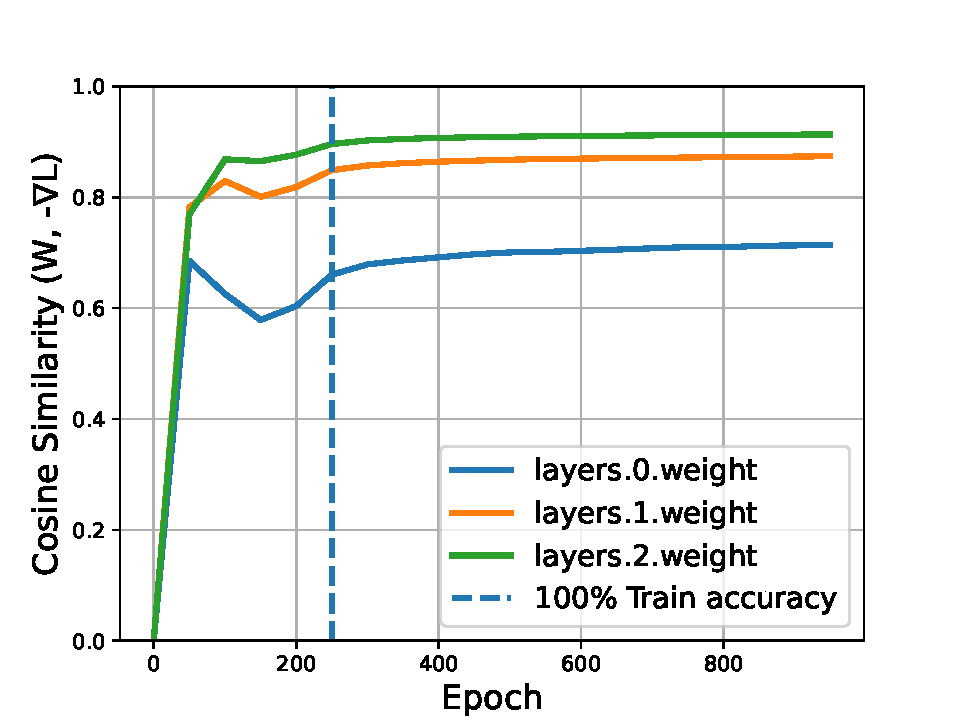
\includegraphics[width=\linewidth]{grokking_iclr_arxiv/figures/nlm_no_bias_mlp.pdf}
    \caption{\vspace{-1mm}MLP without bias terms}
    \label{fig:nmm_no_bias}
\end{subfigure}%
\begin{subfigure}[t]{.33\textwidth}
    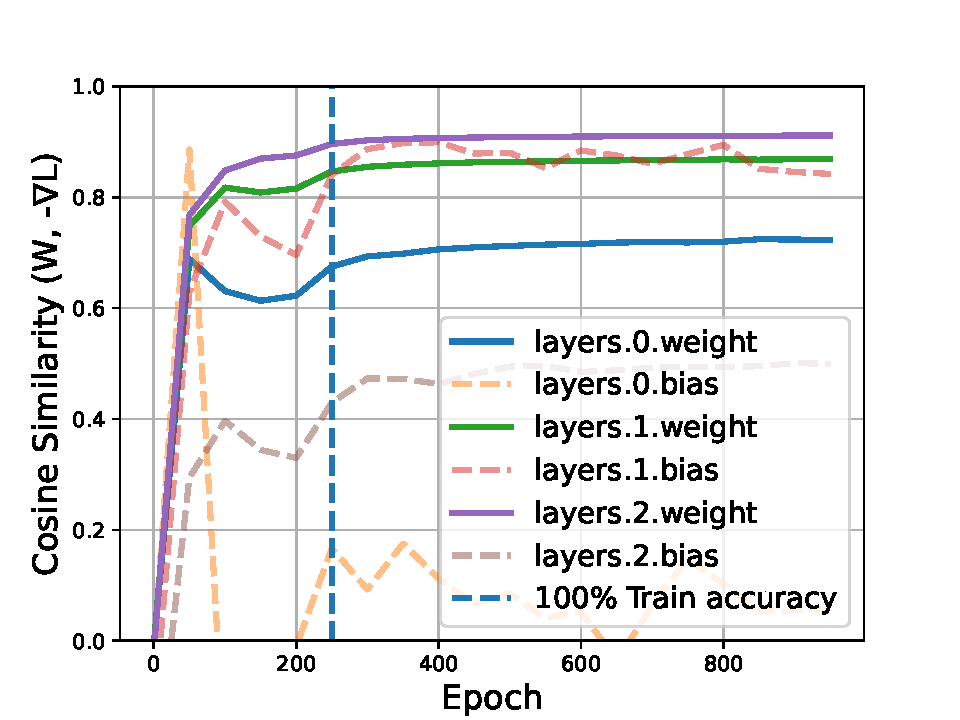
\includegraphics[width=\linewidth]{grokking_iclr_arxiv/figures/nlm_bias_mlp.pdf}
    \caption{\vspace{-1mm}MLP with bias terms}
    \label{fig:nmm_bias}
\end{subfigure}
\begin{subfigure}[t]{.33\textwidth}
    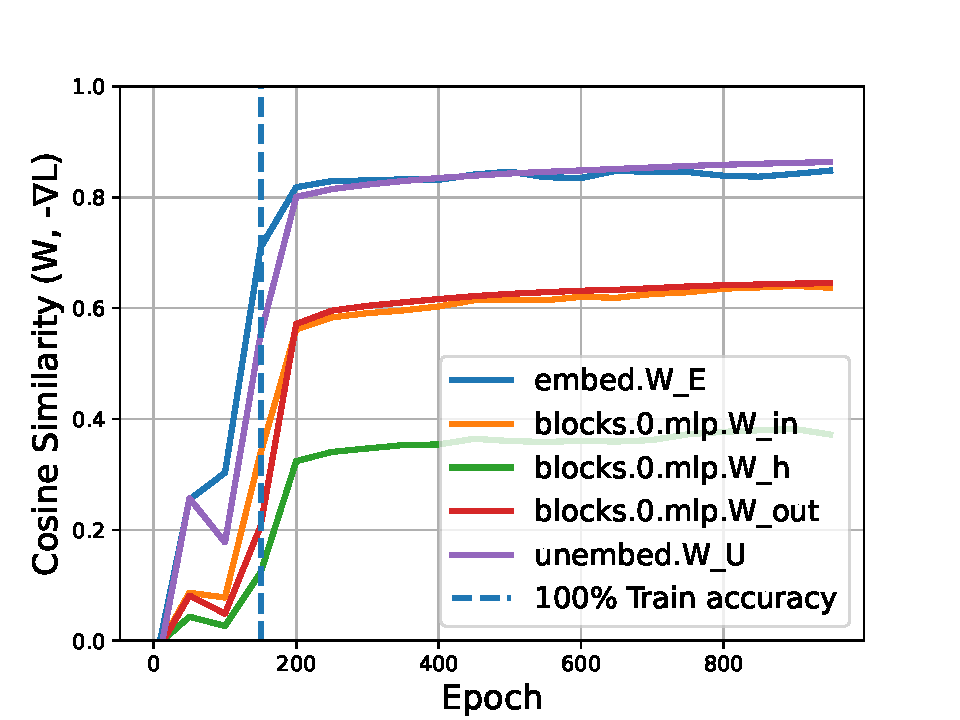
\includegraphics[width=\linewidth]{grokking_iclr_arxiv/figures/nmm_no_bias_transformer.pdf}
    \caption{\vspace{-1mm}Transformer with bias terms}
    \label{fig:nmm_no_bias_transformer}
\end{subfigure}
\vspace{-1mm}
    \caption{MLPs with (\textbf{a}) and without (\textbf{b}) bias terms trained on modular addition receive updates that are significantly aligned with the direction of \nlm beyond the point of overfitting. In (\textbf{c}) we show these results for a selection of parameters for our one layer transformer. We highlight the embed and unembed matrices as well as the weights of the MLP. These are highlighted in the plot using the notation from \cite{elhage2021mathematical}.\vspace{-4mm}}
\label{fig:proof_of_nmm}
\end{figure}
When $f$ is a homogeneous neural network, $L$ corresponds to the number of layers.
\end{dfn}

In the case of homogeneous networks, training beyond 100\% training accuracy, scaling the logits always leads to a decrease in the training loss. Therefore, $d_\mathrm{NLM}(\params)= \alpha\params$ for $\alpha>0$ is an NLM direction, as it results in $f(\params + d_\mathrm{NLM}(\params); \bm{x}) = f((1+\alpha)\params; \bm{x}) = (1+\alpha)^Lf(\params; \bm{x})$, where the second equality follows from \cref{eq:homogeneous}. 

Many neural network architectures, such as ReLU MLPs and transformers without bias terms, are \emph{positively homogeneous} or \emph{approximately homogeneous} in the case of transformers \citep{homogeneous_transformers}. While more complex deep learning models with skip connections and bias terms are not homogeneous, they have been shown to be quasi-homogeneous~\citep{kunin2023asymmetricmaximummarginbias} and in most cases -- including all of the models in this work, the last layer is homogeneous. This means that for non-homogeneous models scaling the weights of the last layer corresponds to a direction of \nlm. 

The fact that the gradients converge to the direction of the weights has been studied in previous works \citep{NEURIPS2020_c76e4b2f, ji2018gradient, ji20182, Lyu2019-sc} to prove that homogeneous networks converge in direction under gradient flow and gradient descent (GD), and they perform normalized margin maximization even beyond the point of $100\%$ training accuracy \citep{Lyu2019-sc}. However, we argue that gradient alignment also results in scaling of the logits which can lead to SC and put an end to the margin maximization described in \cite{Lyu2019-sc}, when working with limited floating point precision. While we study delayed generalization, the link between training trajectories and generalization is already established in prior art~\citep{birdal2021intrinsic,andreeva2024topological}.

\paragraph{Evidence of naïve loss minimization}
In practice, we observe that in MLPs and transformers with and without bias terms, the gradients quickly become aligned with the direction of the weights after the point of overfitting (\cref{fig:proof_of_nmm}). Particularly for the later layers of the models, the cosine similarity between the parameter updates and the NLM direction goes up to 0.9 for the output layers. While models with bias terms are not homogeneous and there is no theoretical guarantee that scaling the weights will reduce the SCE loss, in practice, we observe very similar behaviour in MLPs with (\cref{fig:nmm_bias}) and without (\cref{fig:nmm_no_bias}) bias terms. In the case of a one-layer transformer, the alignment is stronger for the embed and unembed matrices but also substantial for the MLP weights (\cref{fig:nmm_no_bias_transformer}). 












